% !TEX root =  ../main.tex 

\section{Personalized schedules for patients in PRIAS}
\label{sec : pers_schedule_PRIAS}
Our work is motivated by the PRIAS program. To demonstrate how the personalized schedules work, we apply them to the patients enrolled in PRIAS. To this end, we divide the PRIAS data set into training(5264 patients) and demonstration data sets (3 patients). We fit a joint model to the training data set and then use it to create a personalized schedule for patients in demonstration data set. We fit the joint model using the R package JMbayes \citep{rizopoulosJMbayes}, which uses the Bayesian methodology to estimate the model parameters.

\subsection{Fitting the joint model to PRIAS dataset}
\label{subsec : jm_fit_prias}
The training data set $\mathcal{D}^{PRIAS}$ contains information about 5264 prostate cancer patients who satisfied the conditions for enrollment in AS. For every patient the age at the time of induction in AS was recorded. PSA was measured every 3 months for first 2 years and every 6 months thereafter. To detect GR, biopsies were conducted at different time points on the basis of a predetermined schedule as well as PSA-DT as described in Section \ref{sec : introduction}. For the longitudinal analysis of PSA measurements we used $\log_2 PSA$ measurements instead of the raw data. The log transformation was done because the PSA scores take very large values around the time of disease progression. This indicated that the underlying distribution for PSA values was right skewed. The longitudinal sub-model of the joint model we fit is given by:

\begin{equation}
\label{eq : long_model_prias}
\begin{aligned}
\log_2 PSA(t) &= m_i(t) + \varepsilon_i(t), \\
m_i(t) &= (\beta_0 + b_{i0}) + \beta_1 (Age-70) + \beta_2 (Age-70)^2\\ 
&+ \sum_{k=1}^4 \beta_{k+2} B_k(t,\mathcal{K}) + b_{i1} B_7(t, 0.1) + b_{i2} B_8(t, 0.1) \\
\varepsilon_i(t) & \sim N(0, \sigma^2),\\
\end{aligned}
\end{equation}
where, the measurement error $\varepsilon_i(t)$ is assumed normally distributed with mean zero and variance $\sigma^2$, and is independent of the random effects $\boldsymbol{b}_i$. The evolution of PSA levels over time is modeled flexibly using B-splines. For the fixed effects part the spline consists of 3 internal knots. The internal knots are at $\mathcal{K} =\{0.1, 0.5, 4\}$ years, and boundary knots are at 0 and 7 years. For the random effects part there is only 1 internal knot at 0.1 years and the boundary knots are at 0 and 7 years. The choice of knots was based on exploratory analysis as well as on the basis of model selection criteria AIC and BIC. Age of patients was median centered to avoid numerical instabilities while estimating the parameters in the model. For the relative risk sub-model the hazard function we fit is given by:

\begin{equation}
\label{eq : hazard_prias}
h_i(t) = h_0(t) \exp\{\gamma_1 (Age-70)  + \gamma_2 (Age-70)^2  \alpha_1 m_i(t) + \alpha_2 m'_i(t)\}
\end{equation}
where, $\alpha_1$ and $\alpha_2$ are measures of strength of association between hazard of GR and PSA value $m_i(t)$ and PSA velocity $m'_i(t)$, respectively. As mentioned earlier, in PRIAS study PSA-DT is used to decide the schedule of biopsies. However PSA-DT is computed using observed PSA values, and thus interval censoring observed in PRIAS is independent and non informative of underlying health of the patient.

\subsubsection{Parameter Estimates}
\label{subsec : param_estimates_jm_fit_prias}
The posterior parameter estimates $p(\boldsymbol{\theta} \mid \mathcal{D}^{PRIAS})$ for the joint model we fitted to the PRIAS data set are shown in Table \ref{tab : PSA_long} and Table \ref{tab : PSA_survival}. Since the longitudinal evolution of $\log_2 PSA$ is modeled with non-linear terms, the interpretation of the coefficients corresponding to time is not straightforward. In lieu of the interpretation we present the fitted evolution of PSA (Figure \ref{fig : fitted_trend_psa}) over a period of 10 years for a patient who is 70 years old. It can be seen that after the first 6 months the PSA levels steadily increase over the follow up period. Since the model for PSA has only additive terms, this evolution remains same for all patients. The effect of age only affects the baseline PSA score. However it is so small that it can be ignored for all practical purposes.\\

\begin{figure}[!htb]
	\centering
    \captionsetup{justification=centering}
	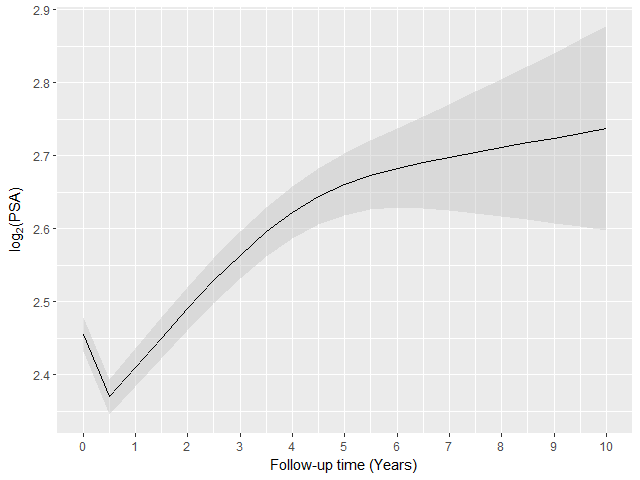
\includegraphics[width=0.8\textwidth]{images/fitted_trend_psa.png}
	\caption{Fitted evolution of $\log_2 PSA$ over a period of 10 years, for a patient who was inducted in AS at the Age of 70 years.}
	\label{fig : fitted_trend_psa}
\end{figure}

\begin{table}[!htb]
\centering
\caption{Longitudinal sub-model estimates for joint model.}
\label{tab : PSA_long}
\captionsetup{justification=centering}
\begin{tabular}{@{}lrrrrr@{}}
\toprule
                                     & Mean   & Std. Dev           & 2.5\%               & 97.5\%              & P              \\ \midrule
Intercept                            &  2.455 & 0.012 & 2.433 & 2.480               & \textless0.000 \\
(Age - 70)                           & 0.003 & 0.001 & 4.9 $\times 10^{-4}$ & 0.006 & 0.032          \\
(Age - 70) $\times$ (Age - 70)       & -0.001 & 1.4 $\times 10^{-4}$ & -0.001 & -3.5 $\times 10^{-4}$ & \textless0.000 \\
Spline: visitTimeYears{[}0, 0.5{]}   & -0.006 & 0.012 & -0.031 & 0.017 & 0.674 \\
Spline: visitTimeYears{[}0.5, 1.2{]} & 0.228 & 0.019 & 0.192 & 0.265               & \textless0.000 \\
Spline: visitTimeYears{[}1.2, 2.5{]} & 0.140 & 0.029 & 0.088 & 0.197               & \textless0.000 \\
Spline: visitTimeYears{[}2.5, 7{]}   & 0.303 & 0.039 & 0.227 & 0.379               & \textless0.000 \\
$\sigma$                               & 0.324 & 0.001 & 0.321 & 0.326              &  \\ \bottomrule
\end{tabular}
\end{table}

For the relative risk sub-model, the parameter estimates in Table \ref{tab : PSA_survival} show that only $\log_2 PSA$ velocity is strongly associated with hazard of GR. For any patient, a unit increase in $\log_2 PSA$ velocity corresponds to a 11 time increase in hazard of GR. The effect of $\log_2 PSA$ value and effect of Age on hazard of GR are small enough to be safely ignored for all practical purposes.

\begin{table}[!htb]
\centering
\caption{Survival sub-model estimates for joint model.}
\captionsetup{justification=centering}
\label{tab : PSA_survival}
\begin{tabular}{@{}lrrrrr@{}}
\toprule
Variable                      & Mean   & Std. Dev & 2.5\%  & 97.5\%                 & P              \\ \midrule
Age - 70                      & 0.037 & 0.006 & 0.025 & 0.0490                  & \textless0.000 \\
(Age - 70) $\times$ (Age - 70) & -0.001 & 0.001 & -0.003 & 1.8 $\times 10^{-4}$ & 0.104          \\
$\log_2 PSA$                  & -0.049 & 0.064 & -0.172 & 0.078 & 0.414         \\
Slope: $\log_2 PSA$           & 2.407 & 0.319 & 1.791 & 3.069 & \textless0.000 \\ \bottomrule
\end{tabular}
\end{table}

\subsection{Demonstration of personalized schedules}
\label{subsec : demo_prias_pers_schedule}
In this section, we demonstrate how the personalized schedules adapt the time of performing a biopsy according to the PSA history and results from repeat biopsies. We demonstrate this using schedules based on expected time of GR and on dynamic risk of GR. For the latter we select $\kappa$ such that Youden's $J$ is maximized (Section \ref{subsubsec : kappa_estimation}). The 3 patients we have chosen for the demonstration data set are part of PRIAS program and never experienced GR. In addition, they have had their repeat biopsies already. Hence a full scale comparison between PRIAS biopsy schedule and personalized scheduling algorithm's biopsy schedule is not possible.\\

The first patient of interest is patient 3174 who was inducted in the PRIAS program at the age of 74 years. The posterior predictive distribution $g(T^*_j)$ for this patient depends only on the PSA measurements since no repeat biopsies were conducted in the time period we considered. The evolution of PSA, time of last biopsy and proposed times of biopsies are shown in Figure \ref{fig : prias_demo_pid_3174}. It can be seen that the PSA remains stable for the first 2 years of follow up, but increases rapidly after that for the next 2 years. Since the hazard of GR depends on PSA velocity (Table\ref{tab : PSA_survival}), the schedule of biopsy based on expected time of GR adjust the times of biopsy according to the steep rise in PSA profile. More specifically, at 2 years the proposed biopsy time is 12.5 years whereas at 4 years it decreases to 5.3 years. For schedules based on dynamic risk of GR, the $\kappa$ value which maximized Youden's $J$ was found to be between 1 and 0.9 at all time points. This survival probability corresponds to times very close to the first biopsy (time 0) due to the sharp rise in PSA values. Hence the biopsies are scheduled much earlier than those based on expected time of GR.\\

\begin{figure}[!htb]
\centering
\captionsetup{justification=centering}
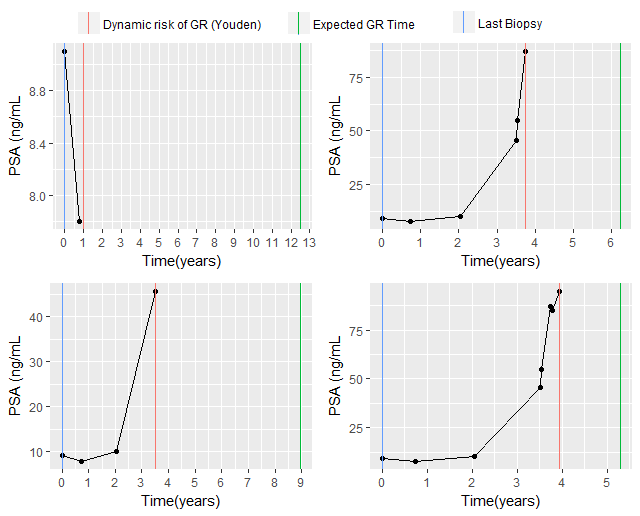
\includegraphics[width=\textwidth]{images/prias_demo/case_3174.png}
\caption{\label{fig : prias_demo_pid_3174} Proposed biopsy times for patient 3174 from PRIAS.}
\end{figure}

It is important to note that for patient 3174, a biopsy scheduled using expected time of GR at year 2 is not as useful as a biopsy scheduled using the same method at year 4. This because $Var_g[T^*_j]$ is considerably lower at year 4 as shown in Figure \ref{fig : variance_pred_dist_3174}. The variance doesn't depend much on number of PSA measurements, but rather on the PSA profile. In the case at hand the variance drops quickly when PSA measurements increase sharply, which is in line with PSA velocity $m'_i(t)$ being a strong predictor of the hazard of GR (Table \ref{tab : PSA_survival}).\\

\begin{figure}[!htb]
    \centering
    \captionsetup{justification=centering}
     \begin{subfigure}[b]{0.45\textwidth}
        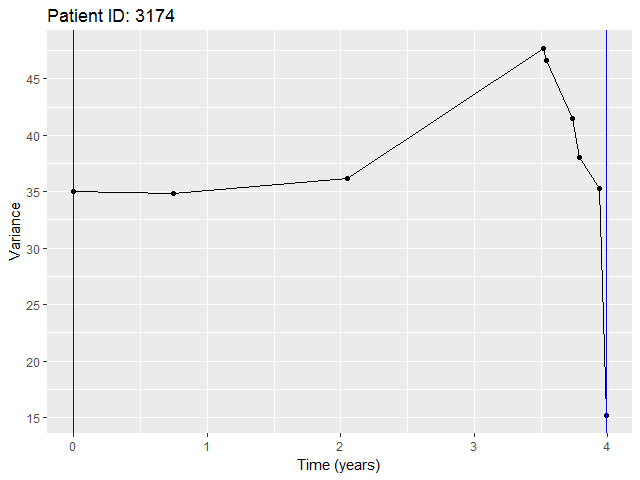
\includegraphics[width=\textwidth]{images/variance/variance_pred_dist_3174.png}
        \caption{Variance of the predictive distribution $g(T^*_j)$ over a period of 4 years for patient 3174. Blue vertical lines indicate biopsies.}
        \label{fig : variance_pred_dist_3174}
    \end{subfigure}
    \begin{subfigure}[b]{0.45\textwidth}
        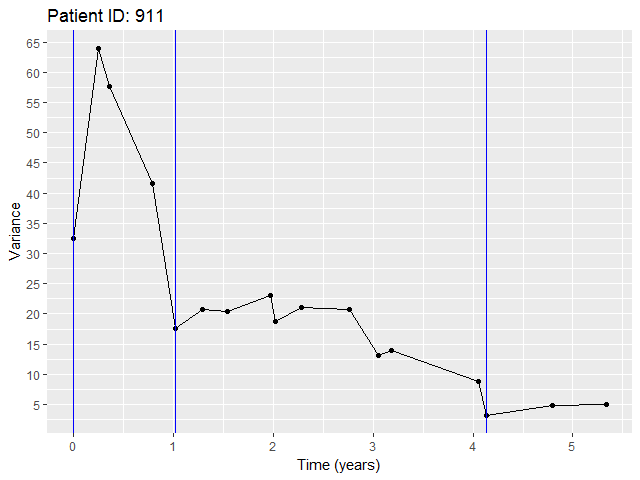
\includegraphics[width=\textwidth]{images/variance/variance_pred_dist_911.png}
        \caption{Variance of the predictive distribution $g(T^*_j)$ over a period of 5 years for patient 911. Blue vertical lines indicate biopsies.}
        \label{fig : variance_pred_dist_911}
    \end{subfigure}
    \label{fig : variance_pred_dist} 
    \caption{Variance of the predictive distribution $g(T^*_j)$}
\end{figure}

The second patient of interest is patient 911. Figure \ref{fig : prias_demo_pid_911} shows the evolution of PSA, time of last biopsy and proposed biopsy times for this patient. Between year 1.5 and year 2, the PSA rises sharply, and accordingly the personalized schedules based on expected time of GR prepone the proposed biopsy time from 14.2 years to 13.8 years. Between year 2 and year 3 the PSA decreases sharply and accordingly the proposed biopsy times are postponed from 13.8 years to 16.6 years. It can also be seen that PSA remains stable up to to year 4. Lastly, because no GR is found at the repeat biopsy performed at 4.1 years, this further leads to postponing of the biopsy times to 18.7 years. As for the schedule based on dynamic risk of GR, the optimal $\kappa$ values are always between 1 and 0.9 at all time points. Correspondingly, the biopsies are conducted very early till a negative biopsy is found at year 4.1, at which we see that the proposed biopsy time is postponed from 3.21 years to 14.8 years, despite the $\kappa$ being equal to 0.98 for both. For patient 911 the biopsies scheduled using $E_g[T^*_j]$ at year 4.1 are expected to be very close to the true GR time of the patient. This because the variance $Var_g[T^*_j]$ is quite low at year 4 as shown in Figure \ref{fig : variance_pred_dist_911}. From the figure it is also evident that the variance decreases considerably each time information about $T^*_j$ from a repeat biopsy is available.\\

\begin{figure}[!htb]
\centering
\captionsetup{justification=centering}
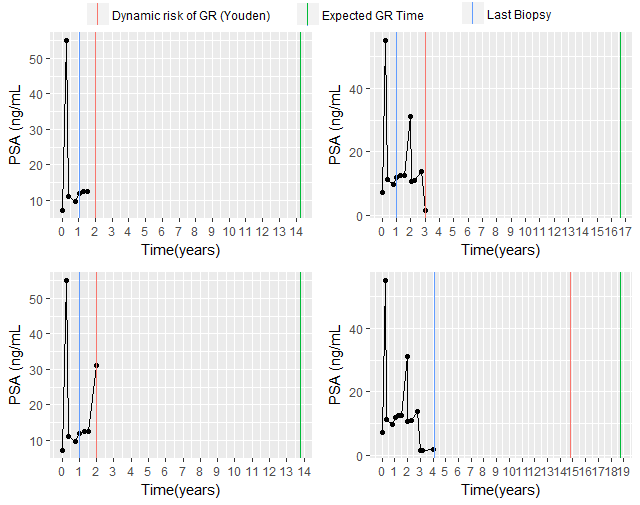
\includegraphics[width=\textwidth]{images/prias_demo/case_911.png}
\caption{\label{fig : prias_demo_pid_911} Proposed biopsy times for patient 911 from PRIAS.}
\end{figure}

From the previous 2 cases we saw that proposed times of biopsy depend on PSA velocity as well as repeat biopsies. Using the profile of patient 2340 we discuss a case where information from PSA levels and repeat biopsies is conflicting. In Figure \ref{fig : prias_demo_pid_2340_yes_biopsy} we can see that the PSA levels for this patient become 4 times between year 1 and year 3, however during the same period a repeat biopsy (year 2.5) was found to be negative. Correspondingly, the personalized schedule based on expected time of GR postpone the time of next biopsy from 14.5 to 15 years. However if there were no repeat biopsy conducted, then only the information from rising PSA levels would've been considered. This is shown in Figure \ref{fig : prias_demo_pid_2340_no_biopsy}, where we can see that personalized schedule based on expected time of GR prepone the time of next biopsy from 12.5 to 11.5 years. As for dynamic risk of GR, we can see that for the same $\kappa$, the corresponding biopsy time is 3.5 years when results from repeat biopsy are considered and it is 3.25 years when repeat biopsies are ignored.

\begin{figure}[!htb]
    \centering
    \captionsetup{justification=centering}
     \begin{subfigure}[b]{\textwidth}
        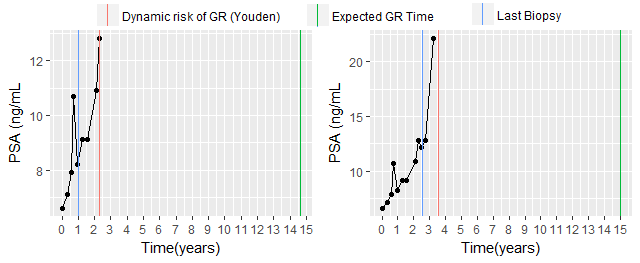
\includegraphics[width=\textwidth]{images/prias_demo/case_2340_yesbiopsy.png}
        \caption{No repeat biopsies is ignored.}
        \label{fig : prias_demo_pid_2340_yes_biopsy}
    \end{subfigure}
    \begin{subfigure}[b]{\textwidth}
        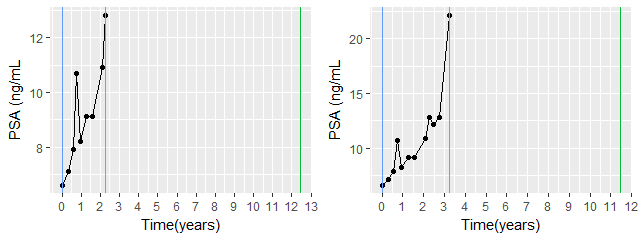
\includegraphics[width=\textwidth]{images/prias_demo/case_2340_nobiopsy.png}
        \caption{All repeat biopsies are ignored.}
        \label{fig : prias_demo_pid_2340_no_biopsy}
    \end{subfigure}
    \label{fig : prias_demo_pid_2340}
    \caption{Proposed biopsy times for patient 2340 from PRIAS.}
\end{figure}